\documentclass[a4paper]{book}
\usepackage{a4wide}
\usepackage{makeidx}
\usepackage{graphicx}
\usepackage{multicol}
\usepackage{float}
\usepackage{listings}
\usepackage{color}
\usepackage{textcomp}
\usepackage{alltt}
\usepackage{times}
\usepackage{ifpdf}
\ifpdf
\usepackage[pdftex,
            pagebackref=true,
            colorlinks=true,
            linkcolor=blue,
            unicode
           ]{hyperref}
\else
\usepackage[ps2pdf,
            pagebackref=true,
            colorlinks=true,
            linkcolor=blue,
            unicode
           ]{hyperref}
\usepackage{pspicture}
\fi
\usepackage[utf8]{inputenc}
\usepackage{doxygen}
\lstset{language=C++,inputencoding=utf8,basicstyle=\footnotesize,breaklines=true,breakatwhitespace=true,tabsize=8,numbers=left }
\makeindex
\setcounter{tocdepth}{3}
\renewcommand{\footrulewidth}{0.4pt}
\begin{document}
\hypersetup{pageanchor=false}
\begin{titlepage}
\vspace*{7cm}
\begin{center}
{\Large jereTanguy }\\
\vspace*{1cm}
{\large Generated by Doxygen 1.6.3}\\
\vspace*{0.5cm}
{\small Wed Oct 5 14:00:24 2011}\\
\end{center}
\end{titlepage}
\clearemptydoublepage
\pagenumbering{roman}
\tableofcontents
\clearemptydoublepage
\pagenumbering{arabic}
\hypersetup{pageanchor=true}
\chapter{Namespace Index}
\section{Namespace List}
Here is a list of all documented namespaces with brief descriptions:\begin{DoxyCompactList}
\item\contentsline{section}{\hyperlink{namespacecell__mdl}{cell\_\-mdl} }{\pageref{namespacecell__mdl}}{}
\end{DoxyCompactList}

\chapter{Data Structure Index}
\section{Class Hierarchy}
This inheritance list is sorted roughly, but not completely, alphabetically:\begin{DoxyCompactList}
\item \contentsline{section}{IntGen}{\pageref{classcell__mdl_1_1_int_gen}}{}
\begin{DoxyCompactList}
\item \contentsline{section}{IntPara}{\pageref{classcell__mdl_1_1_int_para}}{}
\item \contentsline{section}{IntSerial}{\pageref{classcell__mdl_1_1_int_serial}}{}
\end{DoxyCompactList}
\item \contentsline{section}{TissueModel}{\pageref{classcell__mdl_1_1_tissue_model}}{}
\begin{DoxyCompactList}
\item \contentsline{section}{Red3}{\pageref{classcell__mdl_1_1_red3}}{}
\item \contentsline{section}{Red6}{\pageref{classcell__mdl_1_1_red6}}{}
\end{DoxyCompactList}
\end{DoxyCompactList}

\chapter{Data Structure Index}
\section{Data Structures}
Here are the data structures with brief descriptions:\begin{DoxyCompactList}
\item\contentsline{section}{\hyperlink{classcell__mdl_1_1_int_gen}{IntGen} }{\pageref{classcell__mdl_1_1_int_gen}}{}
\item\contentsline{section}{\hyperlink{classcell__mdl_1_1_int_para}{IntPara} }{\pageref{classcell__mdl_1_1_int_para}}{}
\item\contentsline{section}{\hyperlink{classcell__mdl_1_1_int_serial}{IntSerial} }{\pageref{classcell__mdl_1_1_int_serial}}{}
\item\contentsline{section}{\hyperlink{classcell__mdl_1_1_red3}{Red3} }{\pageref{classcell__mdl_1_1_red3}}{}
\item\contentsline{section}{\hyperlink{classcell__mdl_1_1_red6}{Red6} }{\pageref{classcell__mdl_1_1_red6}}{}
\item\contentsline{section}{\hyperlink{classcell__mdl_1_1_tissue_model}{TissueModel} }{\pageref{classcell__mdl_1_1_tissue_model}}{}
\end{DoxyCompactList}

\chapter{Namespace Documentation}
\hypertarget{namespacecell__mdl}{
\section{cell\_\-mdl Namespace Reference}
\label{namespacecell__mdl}\index{cell\_\-mdl@{cell\_\-mdl}}
}
\subsection*{Data Structures}
\begin{DoxyCompactItemize}
\item 
class \hyperlink{classcell__mdl_1_1_tissue_model}{TissueModel}
\item 
class \hyperlink{classcell__mdl_1_1_red3}{Red3}
\item 
class \hyperlink{classcell__mdl_1_1_red6}{Red6}
\item 
class \hyperlink{classcell__mdl_1_1_int_gen}{IntGen}
\item 
class \hyperlink{classcell__mdl_1_1_int_serial}{IntSerial}
\item 
class \hyperlink{classcell__mdl_1_1_int_para}{IntPara}
\end{DoxyCompactItemize}


\subsection{Detailed Description}
\begin{DoxyVerb}Tissue models classes:
Tissuemodel: Generic base class, not a functionnal model by itself.
Red3: Uses reduced 3 vars uterine cell model (J.Laforet).
Red6: Uses reduced 6 vars uterine cell model (S.Rihana).\end{DoxyVerb}
 
\chapter{Data Structure Documentation}
\hypertarget{classcell__mdl_1_1_int_gen}{
\section{IntGen Class Reference}
\label{classcell__mdl_1_1_int_gen}\index{cell\_\-mdl::IntGen@{cell\_\-mdl::IntGen}}
}
Inheritance diagram for IntGen:\begin{figure}[H]
\begin{center}
\leavevmode
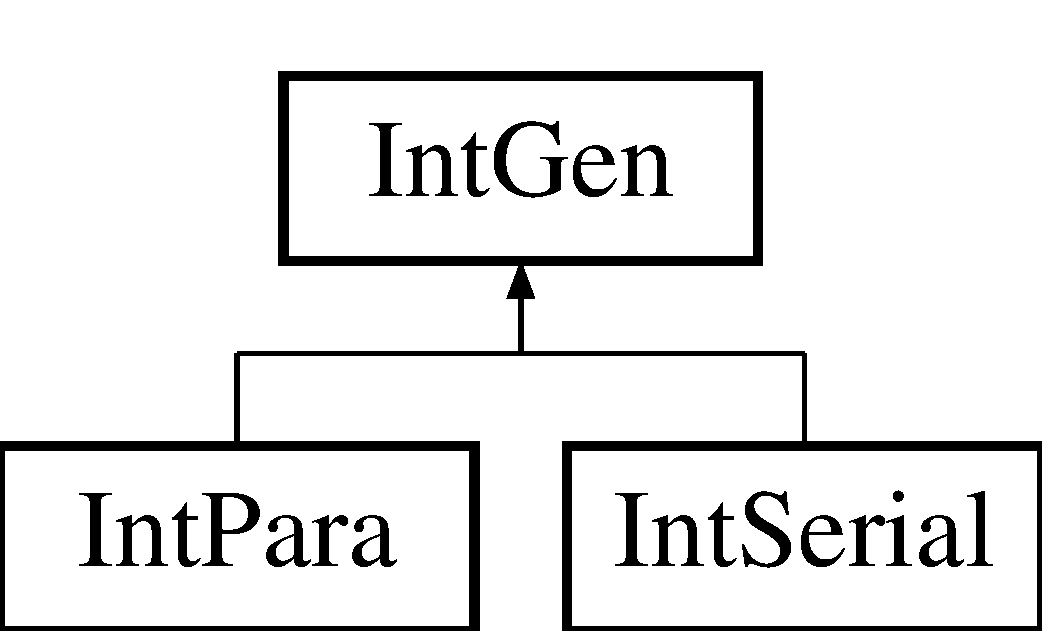
\includegraphics[height=2cm]{classcell__mdl_1_1_int_gen}
\end{center}
\end{figure}
\subsection*{Public Member Functions}
\begin{DoxyCompactItemize}
\item 
def \hyperlink{classcell__mdl_1_1_int_gen_ac775ee34451fdfa742b318538164070e}{\_\-\_\-init\_\-\_\-}
\item 
def \hyperlink{classcell__mdl_1_1_int_gen_aba0970ece8740693d3b82e656500a9c0}{save}
\item 
def \hyperlink{classcell__mdl_1_1_int_gen_a051649d4f6e0c3c1e1e47d8699feb801}{show}
\end{DoxyCompactItemize}
\subsection*{Data Fields}
\begin{DoxyCompactItemize}
\item 
\hypertarget{classcell__mdl_1_1_int_gen_ad6686534e0ed181a7fd0878e86f3848a}{
{\bfseries mdl}}
\label{classcell__mdl_1_1_int_gen_ad6686534e0ed181a7fd0878e86f3848a}

\end{DoxyCompactItemize}


\subsection{Detailed Description}
\begin{DoxyVerb}Generic integrator class\end{DoxyVerb}
 

\subsection{Member Function Documentation}
\hypertarget{classcell__mdl_1_1_int_gen_ac775ee34451fdfa742b318538164070e}{
\index{cell\_\-mdl::IntGen@{cell\_\-mdl::IntGen}!\_\-\_\-init\_\-\_\-@{\_\-\_\-init\_\-\_\-}}
\index{\_\-\_\-init\_\-\_\-@{\_\-\_\-init\_\-\_\-}!cell_mdl::IntGen@{cell\_\-mdl::IntGen}}
\subsubsection[{\_\-\_\-init\_\-\_\-}]{\setlength{\rightskip}{0pt plus 5cm}def \_\-\_\-init\_\-\_\- ( {\em self}, \/   {\em mdl})}}
\label{classcell__mdl_1_1_int_gen_ac775ee34451fdfa742b318538164070e}
\begin{DoxyVerb}The constructor.
mdl : model (of class Red3 or Red6)
\end{DoxyVerb}
 

Reimplemented in \hyperlink{classcell__mdl_1_1_int_serial_ac775ee34451fdfa742b318538164070e}{IntSerial}, and \hyperlink{classcell__mdl_1_1_int_para_ac775ee34451fdfa742b318538164070e}{IntPara}.

\hypertarget{classcell__mdl_1_1_int_gen_aba0970ece8740693d3b82e656500a9c0}{
\index{cell\_\-mdl::IntGen@{cell\_\-mdl::IntGen}!save@{save}}
\index{save@{save}!cell_mdl::IntGen@{cell\_\-mdl::IntGen}}
\subsubsection[{save}]{\setlength{\rightskip}{0pt plus 5cm}def save ( {\em self}, \/   {\em filename})}}
\label{classcell__mdl_1_1_int_gen_aba0970ece8740693d3b82e656500a9c0}
\begin{DoxyVerb}save t and Vm using the method numpy.savez\end{DoxyVerb}
 \hypertarget{classcell__mdl_1_1_int_gen_a051649d4f6e0c3c1e1e47d8699feb801}{
\index{cell\_\-mdl::IntGen@{cell\_\-mdl::IntGen}!show@{show}}
\index{show@{show}!cell_mdl::IntGen@{cell\_\-mdl::IntGen}}
\subsubsection[{show}]{\setlength{\rightskip}{0pt plus 5cm}def show ( {\em self})}}
\label{classcell__mdl_1_1_int_gen_a051649d4f6e0c3c1e1e47d8699feb801}
\begin{DoxyVerb}show Vm in a graph. Works for 1D projects only\end{DoxyVerb}
 

The documentation for this class was generated from the following file:\begin{DoxyCompactItemize}
\item 
/home/tanguy/git/jereTanguy/cell\_\-mdl.py\end{DoxyCompactItemize}

\hypertarget{classcell__mdl_1_1_int_para}{
\section{IntPara Class Reference}
\label{classcell__mdl_1_1_int_para}\index{cell\_\-mdl::IntPara@{cell\_\-mdl::IntPara}}
}
Inheritance diagram for IntPara:\begin{figure}[H]
\begin{center}
\leavevmode
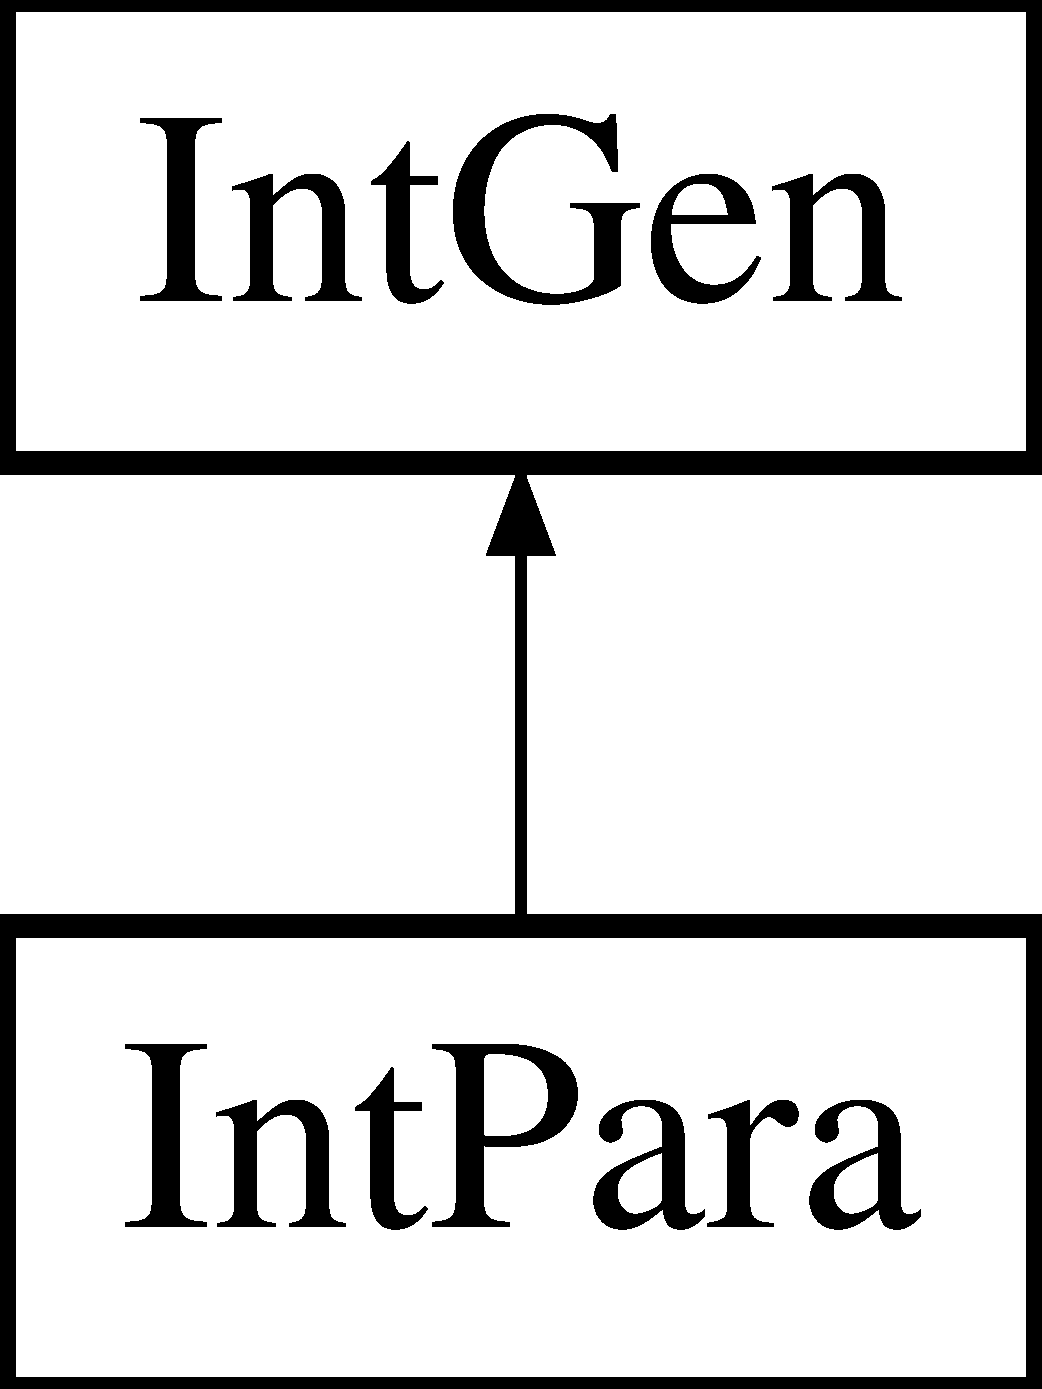
\includegraphics[height=2cm]{classcell__mdl_1_1_int_para}
\end{center}
\end{figure}
\subsection*{Public Member Functions}
\begin{DoxyCompactItemize}
\item 
def \hyperlink{classcell__mdl_1_1_int_para_ac775ee34451fdfa742b318538164070e}{\_\-\_\-init\_\-\_\-}
\item 
def \hyperlink{classcell__mdl_1_1_int_para_aaa2084b96999fb1734fd2f330bfa01a6}{compute}
\end{DoxyCompactItemize}
\subsection*{Data Fields}
\begin{DoxyCompactItemize}
\item 
\hypertarget{classcell__mdl_1_1_int_para_a6838f02691e22b3e6bc338e61f647d52}{
{\bfseries view}}
\label{classcell__mdl_1_1_int_para_a6838f02691e22b3e6bc338e61f647d52}

\item 
\hypertarget{classcell__mdl_1_1_int_para_a5d50b03d9e70ea73ca7ef3abe59b5d50}{
{\bfseries nbx}}
\label{classcell__mdl_1_1_int_para_a5d50b03d9e70ea73ca7ef3abe59b5d50}

\item 
\hypertarget{classcell__mdl_1_1_int_para_a673c0649f4acd57528b5ddf3e3b4fd6b}{
{\bfseries nby}}
\label{classcell__mdl_1_1_int_para_a673c0649f4acd57528b5ddf3e3b4fd6b}

\item 
\hypertarget{classcell__mdl_1_1_int_para_aaccc9105df5383111407fd5b41255e23}{
{\bfseries t}}
\label{classcell__mdl_1_1_int_para_aaccc9105df5383111407fd5b41255e23}

\item 
\hypertarget{classcell__mdl_1_1_int_para_ae2db27d1cd25ddde897eb53858084365}{
{\bfseries Vm}}
\label{classcell__mdl_1_1_int_para_ae2db27d1cd25ddde897eb53858084365}

\end{DoxyCompactItemize}


\subsection{Detailed Description}
\begin{DoxyVerb}Integrator class using parallel computation\end{DoxyVerb}
 

\subsection{Member Function Documentation}
\hypertarget{classcell__mdl_1_1_int_para_ac775ee34451fdfa742b318538164070e}{
\index{cell\_\-mdl::IntPara@{cell\_\-mdl::IntPara}!\_\-\_\-init\_\-\_\-@{\_\-\_\-init\_\-\_\-}}
\index{\_\-\_\-init\_\-\_\-@{\_\-\_\-init\_\-\_\-}!cell_mdl::IntPara@{cell\_\-mdl::IntPara}}
\subsubsection[{\_\-\_\-init\_\-\_\-}]{\setlength{\rightskip}{0pt plus 5cm}def \_\-\_\-init\_\-\_\- ( {\em self}, \/   {\em mdl})}}
\label{classcell__mdl_1_1_int_para_ac775ee34451fdfa742b318538164070e}
\begin{DoxyVerb}The constructor.
mdl : model (of class Red3 or Red6)
\end{DoxyVerb}
 

Reimplemented from \hyperlink{classcell__mdl_1_1_int_gen_ac775ee34451fdfa742b318538164070e}{IntGen}.

\hypertarget{classcell__mdl_1_1_int_para_aaa2084b96999fb1734fd2f330bfa01a6}{
\index{cell\_\-mdl::IntPara@{cell\_\-mdl::IntPara}!compute@{compute}}
\index{compute@{compute}!cell_mdl::IntPara@{cell\_\-mdl::IntPara}}
\subsubsection[{compute}]{\setlength{\rightskip}{0pt plus 5cm}def compute ( {\em self}, \/   {\em tmax} = {\ttfamily 500}, \/   {\em stimCoord} = {\ttfamily \mbox{[}0}, \/   {\em stimCoord2} = {\ttfamily \mbox{[}0})}}
\label{classcell__mdl_1_1_int_para_aaa2084b96999fb1734fd2f330bfa01a6}
\begin{DoxyVerb}Compute.
tmax : maximum duration (in ms)
stimCoord,stimCoord2 : Coordinates of the stimulations
\end{DoxyVerb}
 

The documentation for this class was generated from the following file:\begin{DoxyCompactItemize}
\item 
/home/tanguy/git/jereTanguy/cell\_\-mdl.py\end{DoxyCompactItemize}

\hypertarget{classcell__mdl_1_1_int_serial}{
\section{IntSerial Class Reference}
\label{classcell__mdl_1_1_int_serial}\index{cell\_\-mdl::IntSerial@{cell\_\-mdl::IntSerial}}
}
Inheritance diagram for IntSerial:\begin{figure}[H]
\begin{center}
\leavevmode
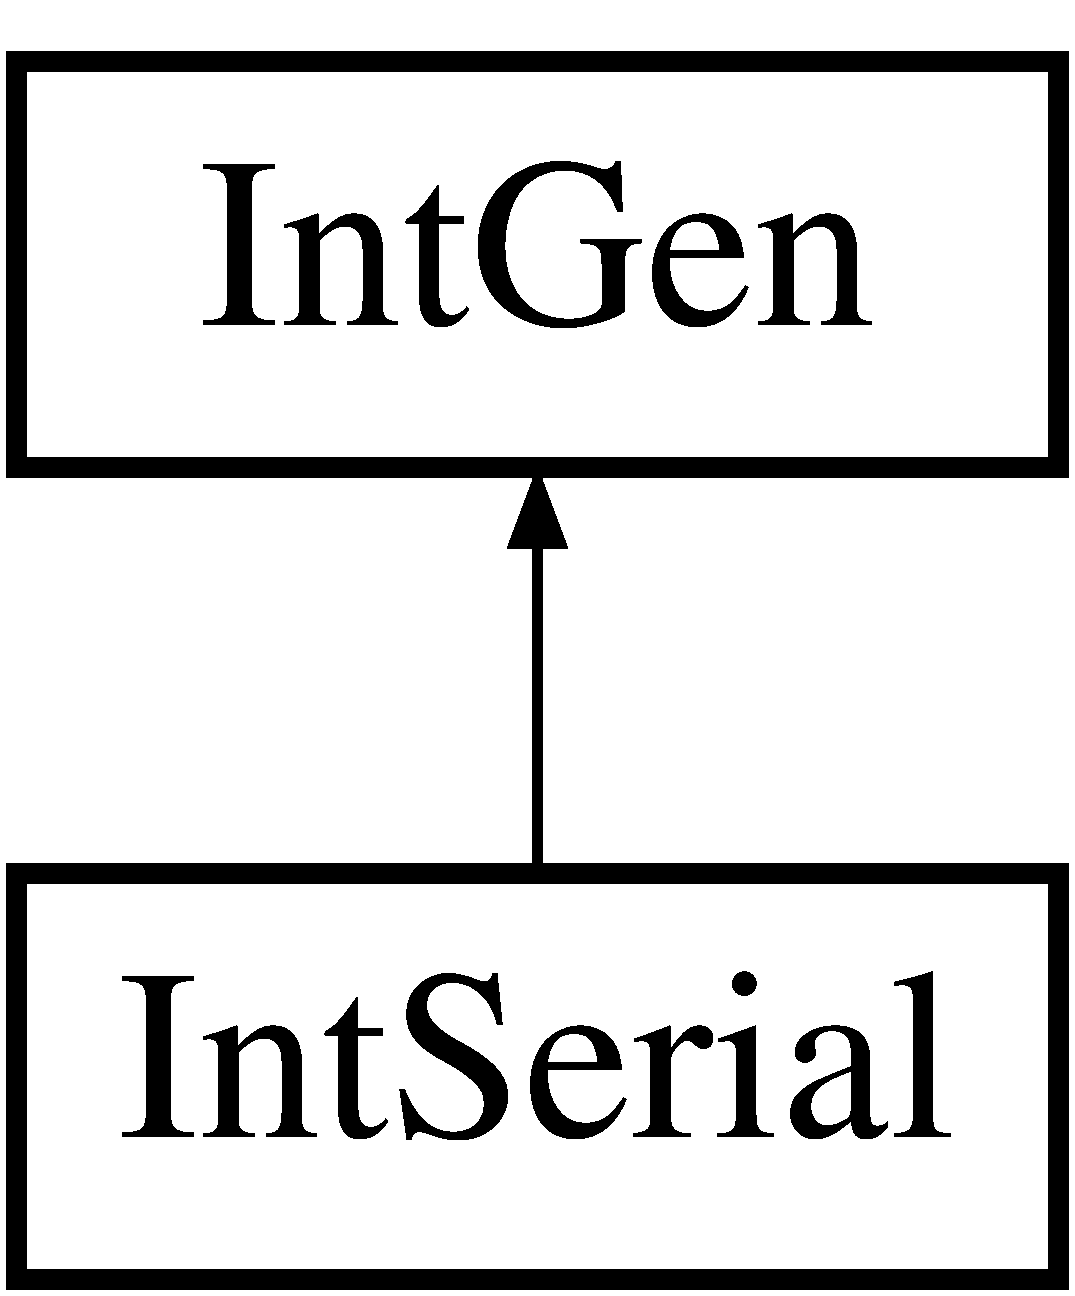
\includegraphics[height=2cm]{classcell__mdl_1_1_int_serial}
\end{center}
\end{figure}
\subsection*{Public Member Functions}
\begin{DoxyCompactItemize}
\item 
def \hyperlink{classcell__mdl_1_1_int_serial_ac775ee34451fdfa742b318538164070e}{\_\-\_\-init\_\-\_\-}
\item 
def \hyperlink{classcell__mdl_1_1_int_serial_aaa2084b96999fb1734fd2f330bfa01a6}{compute}
\end{DoxyCompactItemize}
\subsection*{Data Fields}
\begin{DoxyCompactItemize}
\item 
\hypertarget{classcell__mdl_1_1_int_serial_a536f1b0a72368eae0f278666b6a196eb}{
{\bfseries decim}}
\label{classcell__mdl_1_1_int_serial_a536f1b0a72368eae0f278666b6a196eb}

\item 
\hypertarget{classcell__mdl_1_1_int_serial_a770f288d3048ff6cbee9faa0969fd6b0}{
{\bfseries dt}}
\label{classcell__mdl_1_1_int_serial_a770f288d3048ff6cbee9faa0969fd6b0}

\item 
\hypertarget{classcell__mdl_1_1_int_serial_aaccc9105df5383111407fd5b41255e23}{
{\bfseries t}}
\label{classcell__mdl_1_1_int_serial_aaccc9105df5383111407fd5b41255e23}

\item 
\hypertarget{classcell__mdl_1_1_int_serial_ae2db27d1cd25ddde897eb53858084365}{
{\bfseries Vm}}
\label{classcell__mdl_1_1_int_serial_ae2db27d1cd25ddde897eb53858084365}

\end{DoxyCompactItemize}


\subsection{Detailed Description}
\begin{DoxyVerb}Integrator class using serial computation\end{DoxyVerb}
 

\subsection{Member Function Documentation}
\hypertarget{classcell__mdl_1_1_int_serial_ac775ee34451fdfa742b318538164070e}{
\index{cell\_\-mdl::IntSerial@{cell\_\-mdl::IntSerial}!\_\-\_\-init\_\-\_\-@{\_\-\_\-init\_\-\_\-}}
\index{\_\-\_\-init\_\-\_\-@{\_\-\_\-init\_\-\_\-}!cell_mdl::IntSerial@{cell\_\-mdl::IntSerial}}
\subsubsection[{\_\-\_\-init\_\-\_\-}]{\setlength{\rightskip}{0pt plus 5cm}def \_\-\_\-init\_\-\_\- ( {\em self}, \/   {\em mdl})}}
\label{classcell__mdl_1_1_int_serial_ac775ee34451fdfa742b318538164070e}
\begin{DoxyVerb}The constructor.
mdl : model (of class Red3 or Red6)
\end{DoxyVerb}
 

Reimplemented from \hyperlink{classcell__mdl_1_1_int_gen_ac775ee34451fdfa742b318538164070e}{IntGen}.

\hypertarget{classcell__mdl_1_1_int_serial_aaa2084b96999fb1734fd2f330bfa01a6}{
\index{cell\_\-mdl::IntSerial@{cell\_\-mdl::IntSerial}!compute@{compute}}
\index{compute@{compute}!cell_mdl::IntSerial@{cell\_\-mdl::IntSerial}}
\subsubsection[{compute}]{\setlength{\rightskip}{0pt plus 5cm}def compute ( {\em self}, \/   {\em tmax} = {\ttfamily 500}, \/   {\em stimCoord} = {\ttfamily \mbox{[}0}, \/   {\em stimCoord2} = {\ttfamily \mbox{[}0})}}
\label{classcell__mdl_1_1_int_serial_aaa2084b96999fb1734fd2f330bfa01a6}
\begin{DoxyVerb}Compute.
tmax : maximum duration (in ms)
stimCoord,stimCoord2 : Coordinates of the stimulations
\end{DoxyVerb}
 

The documentation for this class was generated from the following file:\begin{DoxyCompactItemize}
\item 
/home/tanguy/git/jereTanguy/cell\_\-mdl.py\end{DoxyCompactItemize}

\hypertarget{classcell__mdl_1_1_red3}{
\section{Red3 Class Reference}
\label{classcell__mdl_1_1_red3}\index{cell\_\-mdl::Red3@{cell\_\-mdl::Red3}}
}
Inheritance diagram for Red3:\begin{figure}[H]
\begin{center}
\leavevmode
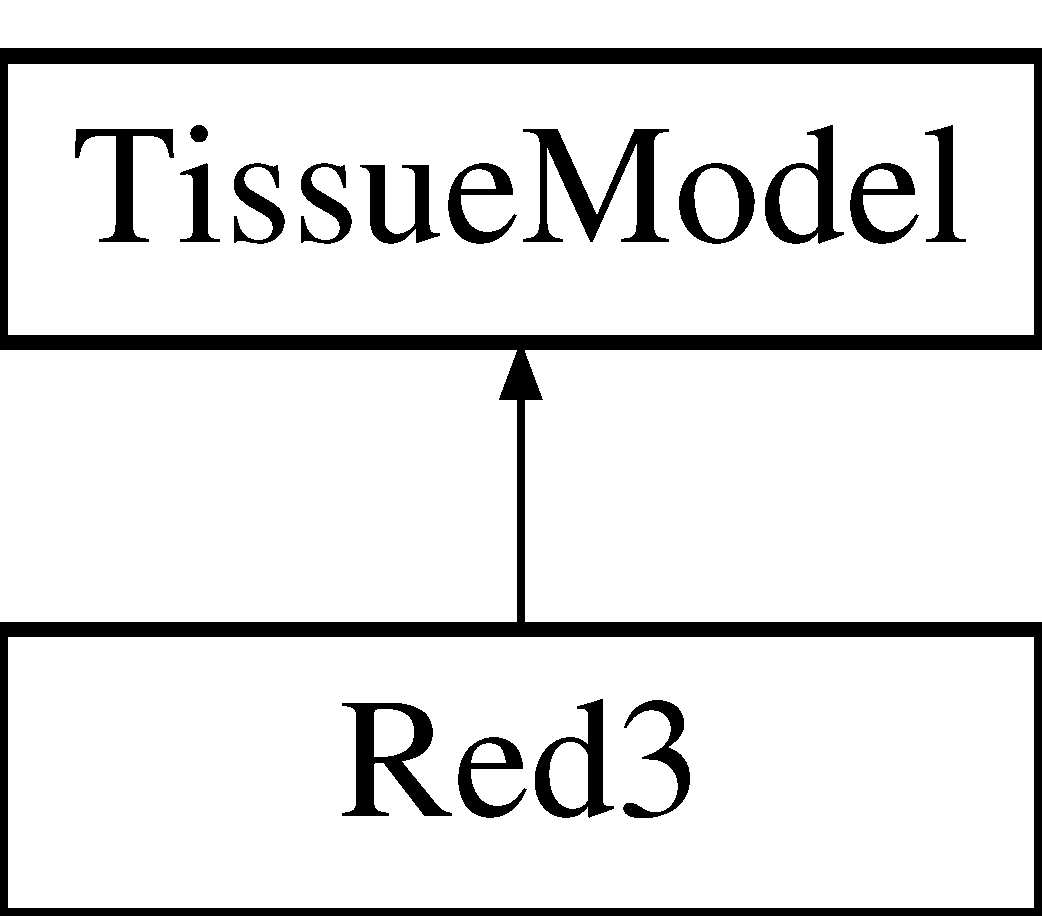
\includegraphics[height=2cm]{classcell__mdl_1_1_red3}
\end{center}
\end{figure}
\subsection*{Public Member Functions}
\begin{DoxyCompactItemize}
\item 
def \hyperlink{classcell__mdl_1_1_red3_ac775ee34451fdfa742b318538164070e}{\_\-\_\-init\_\-\_\-}
\item 
def \hyperlink{classcell__mdl_1_1_red3_ad67701a6bb599a16a9eb386aa1cd4328}{derivT}
\end{DoxyCompactItemize}
\subsection*{Data Fields}
\begin{DoxyCompactItemize}
\item 
\hypertarget{classcell__mdl_1_1_red3_aecc08eb2224f119032db900c1d7e9a91}{
{\bfseries varlist}}
\label{classcell__mdl_1_1_red3_aecc08eb2224f119032db900c1d7e9a91}

\item 
\hypertarget{classcell__mdl_1_1_red3_aa5998168cabfb2b2e41151349077812c}{
{\bfseries Name}}
\label{classcell__mdl_1_1_red3_aa5998168cabfb2b2e41151349077812c}

\item 
\hypertarget{classcell__mdl_1_1_red3_aab898360e554c7fefb318f71655898e8}{
{\bfseries Gk}}
\label{classcell__mdl_1_1_red3_aab898360e554c7fefb318f71655898e8}

\item 
\hypertarget{classcell__mdl_1_1_red3_aba34b7e0d56c4136ff43780cbea6299c}{
{\bfseries Gkca}}
\label{classcell__mdl_1_1_red3_aba34b7e0d56c4136ff43780cbea6299c}

\item 
\hypertarget{classcell__mdl_1_1_red3_a25e10dd28c2495bc36981494521c22a0}{
{\bfseries Gl}}
\label{classcell__mdl_1_1_red3_a25e10dd28c2495bc36981494521c22a0}

\item 
\hypertarget{classcell__mdl_1_1_red3_a3fdafcf75396b6d11bcb8b5b9a600827}{
{\bfseries Kd}}
\label{classcell__mdl_1_1_red3_a3fdafcf75396b6d11bcb8b5b9a600827}

\item 
\hypertarget{classcell__mdl_1_1_red3_a72d54db2b27ce046aab6e6a414c407e9}{
{\bfseries fc}}
\label{classcell__mdl_1_1_red3_a72d54db2b27ce046aab6e6a414c407e9}

\item 
\hypertarget{classcell__mdl_1_1_red3_a62197192f0fbf4e0675eb37be1c4c175}{
{\bfseries alpha}}
\label{classcell__mdl_1_1_red3_a62197192f0fbf4e0675eb37be1c4c175}

\item 
\hypertarget{classcell__mdl_1_1_red3_a991a17ce4af3dedd3e3371db28579d47}{
{\bfseries Kca}}
\label{classcell__mdl_1_1_red3_a991a17ce4af3dedd3e3371db28579d47}

\item 
\hypertarget{classcell__mdl_1_1_red3_a5f34de0b936acd806815dccdd70a8766}{
{\bfseries El}}
\label{classcell__mdl_1_1_red3_a5f34de0b936acd806815dccdd70a8766}

\item 
\hypertarget{classcell__mdl_1_1_red3_acbf7f480b7d4d43df681879f7cccbd77}{
{\bfseries Ek}}
\label{classcell__mdl_1_1_red3_acbf7f480b7d4d43df681879f7cccbd77}

\item 
\hypertarget{classcell__mdl_1_1_red3_a717bbb86c8afe169ebbf84b4f01998a8}{
{\bfseries Gca2}}
\label{classcell__mdl_1_1_red3_a717bbb86c8afe169ebbf84b4f01998a8}

\item 
\hypertarget{classcell__mdl_1_1_red3_aa783a2b833729df8570b0f66be441529}{
{\bfseries vca2}}
\label{classcell__mdl_1_1_red3_aa783a2b833729df8570b0f66be441529}

\item 
\hypertarget{classcell__mdl_1_1_red3_a99e0a0d42db1d5146e1db7d9def4d875}{
{\bfseries Rca}}
\label{classcell__mdl_1_1_red3_a99e0a0d42db1d5146e1db7d9def4d875}

\item 
\hypertarget{classcell__mdl_1_1_red3_a069197a6f80b4b40b374f98744011311}{
{\bfseries Jbase}}
\label{classcell__mdl_1_1_red3_a069197a6f80b4b40b374f98744011311}

\item 
\hypertarget{classcell__mdl_1_1_red3_a90011e7d69aec5376e286b72ae9e0730}{
{\bfseries dY}}
\label{classcell__mdl_1_1_red3_a90011e7d69aec5376e286b72ae9e0730}

\end{DoxyCompactItemize}


\subsection{Detailed Description}
\begin{DoxyVerb}Cellular and tissular model Red3\end{DoxyVerb}
 

\subsection{Member Function Documentation}
\hypertarget{classcell__mdl_1_1_red3_ac775ee34451fdfa742b318538164070e}{
\index{cell\_\-mdl::Red3@{cell\_\-mdl::Red3}!\_\-\_\-init\_\-\_\-@{\_\-\_\-init\_\-\_\-}}
\index{\_\-\_\-init\_\-\_\-@{\_\-\_\-init\_\-\_\-}!cell_mdl::Red3@{cell\_\-mdl::Red3}}
\subsubsection[{\_\-\_\-init\_\-\_\-}]{\setlength{\rightskip}{0pt plus 5cm}def \_\-\_\-init\_\-\_\- ( {\em self}, \/   {\em Nx}, \/   {\em Ny} = {\ttfamily 0}, \/   {\em Nz} = {\ttfamily 0}, \/   {\em noise} = {\ttfamily 0.0}, \/   {\em borders} = {\ttfamily \mbox{[}True}, \/   {\em True}, \/   {\em True}, \/   {\em True}, \/   {\em True}, \/   {\em True})}}
\label{classcell__mdl_1_1_red3_ac775ee34451fdfa742b318538164070e}
\begin{DoxyVerb}Model init.\end{DoxyVerb}
 \hypertarget{classcell__mdl_1_1_red3_ad67701a6bb599a16a9eb386aa1cd4328}{
\index{cell\_\-mdl::Red3@{cell\_\-mdl::Red3}!derivT@{derivT}}
\index{derivT@{derivT}!cell_mdl::Red3@{cell\_\-mdl::Red3}}
\subsubsection[{derivT}]{\setlength{\rightskip}{0pt plus 5cm}def derivT ( {\em self}, \/   {\em dt})}}
\label{classcell__mdl_1_1_red3_ad67701a6bb599a16a9eb386aa1cd4328}
\begin{DoxyVerb}Computes temporal derivative for red3 model.\end{DoxyVerb}
 

The documentation for this class was generated from the following file:\begin{DoxyCompactItemize}
\item 
/home/tanguy/git/jereTanguy/cell\_\-mdl.py\end{DoxyCompactItemize}

\hypertarget{classcell__mdl_1_1_red6}{
\section{Red6 Class Reference}
\label{classcell__mdl_1_1_red6}\index{cell\_\-mdl::Red6@{cell\_\-mdl::Red6}}
}
Inheritance diagram for Red6:\begin{figure}[H]
\begin{center}
\leavevmode
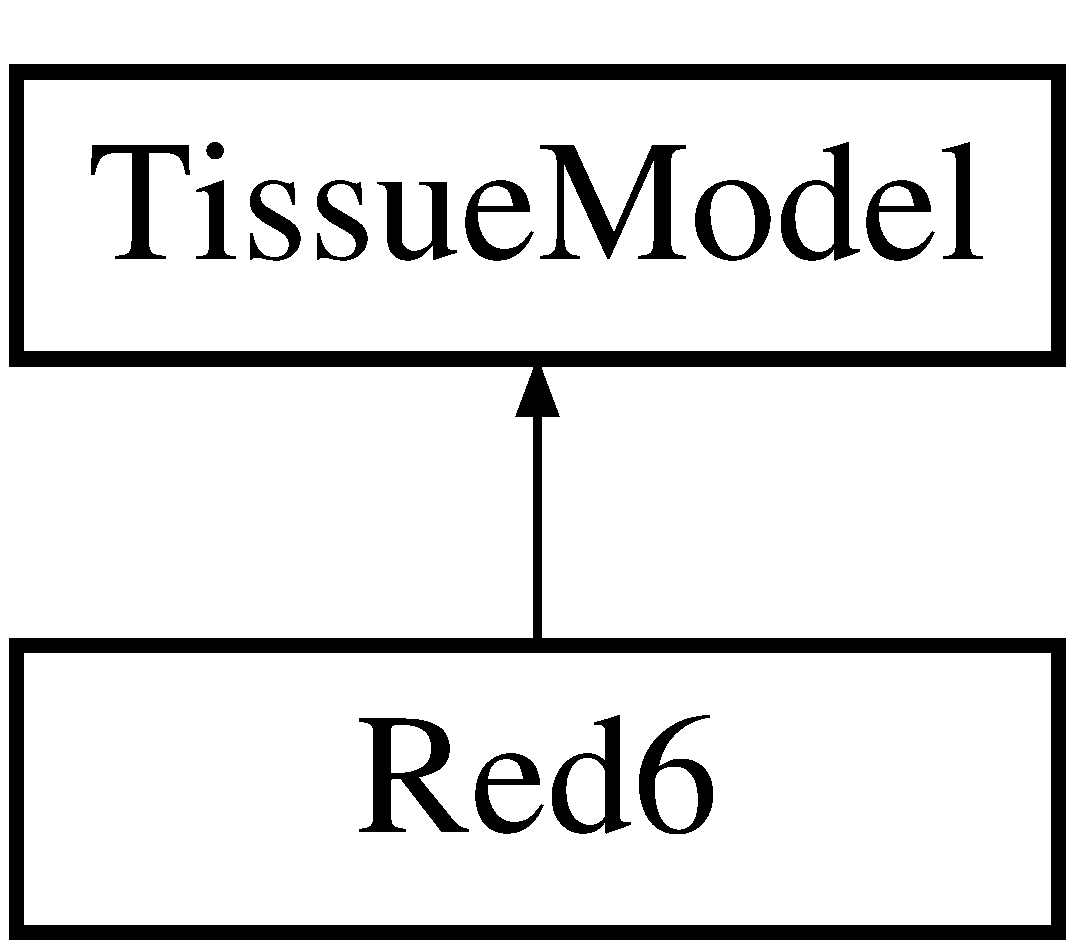
\includegraphics[height=2cm]{classcell__mdl_1_1_red6}
\end{center}
\end{figure}
\subsection*{Public Member Functions}
\begin{DoxyCompactItemize}
\item 
def \hyperlink{classcell__mdl_1_1_red6_ac775ee34451fdfa742b318538164070e}{\_\-\_\-init\_\-\_\-}
\item 
def \hyperlink{classcell__mdl_1_1_red6_ad67701a6bb599a16a9eb386aa1cd4328}{derivT}
\end{DoxyCompactItemize}
\subsection*{Data Fields}
\begin{DoxyCompactItemize}
\item 
\hypertarget{classcell__mdl_1_1_red6_aecc08eb2224f119032db900c1d7e9a91}{
{\bfseries varlist}}
\label{classcell__mdl_1_1_red6_aecc08eb2224f119032db900c1d7e9a91}

\item 
\hypertarget{classcell__mdl_1_1_red6_aa5998168cabfb2b2e41151349077812c}{
{\bfseries Name}}
\label{classcell__mdl_1_1_red6_aa5998168cabfb2b2e41151349077812c}

\item 
\hypertarget{classcell__mdl_1_1_red6_a9c83c0683c6db2817ae77a1a043127de}{
{\bfseries Gca}}
\label{classcell__mdl_1_1_red6_a9c83c0683c6db2817ae77a1a043127de}

\item 
\hypertarget{classcell__mdl_1_1_red6_aab898360e554c7fefb318f71655898e8}{
{\bfseries Gk}}
\label{classcell__mdl_1_1_red6_aab898360e554c7fefb318f71655898e8}

\item 
\hypertarget{classcell__mdl_1_1_red6_aba34b7e0d56c4136ff43780cbea6299c}{
{\bfseries Gkca}}
\label{classcell__mdl_1_1_red6_aba34b7e0d56c4136ff43780cbea6299c}

\item 
\hypertarget{classcell__mdl_1_1_red6_a25e10dd28c2495bc36981494521c22a0}{
{\bfseries Gl}}
\label{classcell__mdl_1_1_red6_a25e10dd28c2495bc36981494521c22a0}

\item 
\hypertarget{classcell__mdl_1_1_red6_a3fdafcf75396b6d11bcb8b5b9a600827}{
{\bfseries Kd}}
\label{classcell__mdl_1_1_red6_a3fdafcf75396b6d11bcb8b5b9a600827}

\item 
\hypertarget{classcell__mdl_1_1_red6_a72d54db2b27ce046aab6e6a414c407e9}{
{\bfseries fc}}
\label{classcell__mdl_1_1_red6_a72d54db2b27ce046aab6e6a414c407e9}

\item 
\hypertarget{classcell__mdl_1_1_red6_a62197192f0fbf4e0675eb37be1c4c175}{
{\bfseries alpha}}
\label{classcell__mdl_1_1_red6_a62197192f0fbf4e0675eb37be1c4c175}

\item 
\hypertarget{classcell__mdl_1_1_red6_a991a17ce4af3dedd3e3371db28579d47}{
{\bfseries Kca}}
\label{classcell__mdl_1_1_red6_a991a17ce4af3dedd3e3371db28579d47}

\item 
\hypertarget{classcell__mdl_1_1_red6_a5f34de0b936acd806815dccdd70a8766}{
{\bfseries El}}
\label{classcell__mdl_1_1_red6_a5f34de0b936acd806815dccdd70a8766}

\item 
\hypertarget{classcell__mdl_1_1_red6_acbf7f480b7d4d43df681879f7cccbd77}{
{\bfseries Ek}}
\label{classcell__mdl_1_1_red6_acbf7f480b7d4d43df681879f7cccbd77}

\item 
\hypertarget{classcell__mdl_1_1_red6_a90011e7d69aec5376e286b72ae9e0730}{
{\bfseries dY}}
\label{classcell__mdl_1_1_red6_a90011e7d69aec5376e286b72ae9e0730}

\end{DoxyCompactItemize}


\subsection{Detailed Description}
\begin{DoxyVerb}Cellular and tissular model Red6\end{DoxyVerb}
 

\subsection{Member Function Documentation}
\hypertarget{classcell__mdl_1_1_red6_ac775ee34451fdfa742b318538164070e}{
\index{cell\_\-mdl::Red6@{cell\_\-mdl::Red6}!\_\-\_\-init\_\-\_\-@{\_\-\_\-init\_\-\_\-}}
\index{\_\-\_\-init\_\-\_\-@{\_\-\_\-init\_\-\_\-}!cell_mdl::Red6@{cell\_\-mdl::Red6}}
\subsubsection[{\_\-\_\-init\_\-\_\-}]{\setlength{\rightskip}{0pt plus 5cm}def \_\-\_\-init\_\-\_\- ( {\em self}, \/   {\em Nx}, \/   {\em Ny} = {\ttfamily 0}, \/   {\em Nz} = {\ttfamily 0}, \/   {\em noise} = {\ttfamily 0.0}, \/   {\em borders} = {\ttfamily \mbox{[}True}, \/   {\em True}, \/   {\em True}, \/   {\em True}, \/   {\em True}, \/   {\em True})}}
\label{classcell__mdl_1_1_red6_ac775ee34451fdfa742b318538164070e}
\begin{DoxyVerb}Model init.\end{DoxyVerb}
 \hypertarget{classcell__mdl_1_1_red6_ad67701a6bb599a16a9eb386aa1cd4328}{
\index{cell\_\-mdl::Red6@{cell\_\-mdl::Red6}!derivT@{derivT}}
\index{derivT@{derivT}!cell_mdl::Red6@{cell\_\-mdl::Red6}}
\subsubsection[{derivT}]{\setlength{\rightskip}{0pt plus 5cm}def derivT ( {\em self}, \/   {\em dt})}}
\label{classcell__mdl_1_1_red6_ad67701a6bb599a16a9eb386aa1cd4328}
\begin{DoxyVerb}Computes temporal derivative for red3 model.\end{DoxyVerb}
 

The documentation for this class was generated from the following file:\begin{DoxyCompactItemize}
\item 
/home/tanguy/git/jereTanguy/cell\_\-mdl.py\end{DoxyCompactItemize}

\hypertarget{classcell__mdl_1_1_tissue_model}{
\section{TissueModel Class Reference}
\label{classcell__mdl_1_1_tissue_model}\index{cell\_\-mdl::TissueModel@{cell\_\-mdl::TissueModel}}
}
Inheritance diagram for TissueModel:\begin{figure}[H]
\begin{center}
\leavevmode
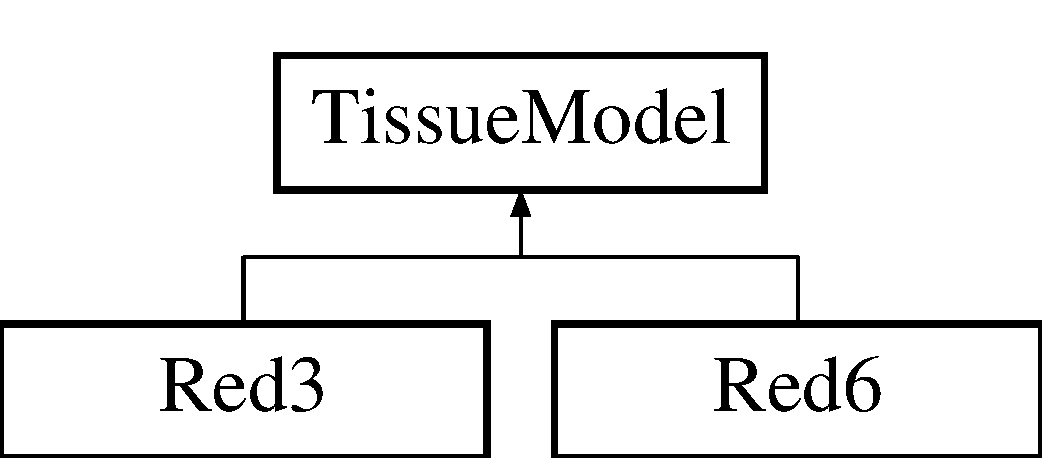
\includegraphics[height=2cm]{classcell__mdl_1_1_tissue_model}
\end{center}
\end{figure}
\subsection*{Public Member Functions}
\begin{DoxyCompactItemize}
\item 
def \hyperlink{classcell__mdl_1_1_tissue_model_ac775ee34451fdfa742b318538164070e}{\_\-\_\-init\_\-\_\-}
\item 
def \hyperlink{classcell__mdl_1_1_tissue_model_a18cbf53eb92c048eacd39a7844d1ec80}{copyparams}
\item 
def \hyperlink{classcell__mdl_1_1_tissue_model_af7fb94e292201b2f2f604451032f38cc}{getlistparams}
\item 
def \hyperlink{classcell__mdl_1_1_tissue_model_ad28a0977f1887b1c30f096d38b28215c}{setlistparams}
\item 
def \hyperlink{classcell__mdl_1_1_tissue_model_ad8b9328939df072e4740cd9a63189744}{\_\-\_\-repr\_\-\_\-}
\item 
\hypertarget{classcell__mdl_1_1_tissue_model_a9cc821f7aefa54284b62f694eac0864d}{
def {\bfseries diff1d}}
\label{classcell__mdl_1_1_tissue_model_a9cc821f7aefa54284b62f694eac0864d}

\item 
\hypertarget{classcell__mdl_1_1_tissue_model_ac60b77951425af4c19b532efbfae57ad}{
def {\bfseries diff2d}}
\label{classcell__mdl_1_1_tissue_model_ac60b77951425af4c19b532efbfae57ad}

\item 
\hypertarget{classcell__mdl_1_1_tissue_model_a3be5bc7f26e6d6c029ec1d4674f899a2}{
def {\bfseries diff3d}}
\label{classcell__mdl_1_1_tissue_model_a3be5bc7f26e6d6c029ec1d4674f899a2}

\item 
def \hyperlink{classcell__mdl_1_1_tissue_model_aa124f33cab14b4466d10c00c8ec82875}{plotstate}
\end{DoxyCompactItemize}
\subsection*{Data Fields}
\begin{DoxyCompactItemize}
\item 
\hypertarget{classcell__mdl_1_1_tissue_model_aa5998168cabfb2b2e41151349077812c}{
{\bfseries Name}}
\label{classcell__mdl_1_1_tissue_model_aa5998168cabfb2b2e41151349077812c}

\item 
\hypertarget{classcell__mdl_1_1_tissue_model_a7ae6d89c76991ba249eb7a977ea81dcb}{
{\bfseries Padding}}
\label{classcell__mdl_1_1_tissue_model_a7ae6d89c76991ba249eb7a977ea81dcb}

\item 
\hypertarget{classcell__mdl_1_1_tissue_model_a70c092a6aebace0b1ea406e14da78a40}{
{\bfseries time}}
\label{classcell__mdl_1_1_tissue_model_a70c092a6aebace0b1ea406e14da78a40}

\item 
\hypertarget{classcell__mdl_1_1_tissue_model_a5c7e4f16622600cb52580b191565e2dd}{
{\bfseries Nx}}
\label{classcell__mdl_1_1_tissue_model_a5c7e4f16622600cb52580b191565e2dd}

\item 
\hypertarget{classcell__mdl_1_1_tissue_model_ac1452fdfd6ea1c8c005ac90bbfa62011}{
{\bfseries Ny}}
\label{classcell__mdl_1_1_tissue_model_ac1452fdfd6ea1c8c005ac90bbfa62011}

\item 
\hypertarget{classcell__mdl_1_1_tissue_model_af3ec54a0e6bc4935a13fb520b7d7df6e}{
{\bfseries Nz}}
\label{classcell__mdl_1_1_tissue_model_af3ec54a0e6bc4935a13fb520b7d7df6e}

\item 
\hypertarget{classcell__mdl_1_1_tissue_model_a0867f43e27585e019c13f7f4b7c4ab6b}{
{\bfseries Y}}
\label{classcell__mdl_1_1_tissue_model_a0867f43e27585e019c13f7f4b7c4ab6b}

\item 
\hypertarget{classcell__mdl_1_1_tissue_model_a5d76cc2129e79ba1941d2cc2f53b9e8e}{
{\bfseries mask}}
\label{classcell__mdl_1_1_tissue_model_a5d76cc2129e79ba1941d2cc2f53b9e8e}

\item 
\hypertarget{classcell__mdl_1_1_tissue_model_a221651ae8493aa5d8c9a925929979c19}{
{\bfseries Dx}}
\label{classcell__mdl_1_1_tissue_model_a221651ae8493aa5d8c9a925929979c19}

\item 
\hypertarget{classcell__mdl_1_1_tissue_model_ae229cbeebddbd49551c4e0555c9623de}{
{\bfseries Dy}}
\label{classcell__mdl_1_1_tissue_model_ae229cbeebddbd49551c4e0555c9623de}

\item 
\hypertarget{classcell__mdl_1_1_tissue_model_a8db728ad14a2f6575482e58156c1088d}{
{\bfseries Dz}}
\label{classcell__mdl_1_1_tissue_model_a8db728ad14a2f6575482e58156c1088d}

\item 
\hypertarget{classcell__mdl_1_1_tissue_model_a11fbc4b6e768e8a1c81399d7341554a8}{
{\bfseries derivS}}
\label{classcell__mdl_1_1_tissue_model_a11fbc4b6e768e8a1c81399d7341554a8}

\item 
\hypertarget{classcell__mdl_1_1_tissue_model_acb95449a94688af33f6e9bb090cf2936}{
{\bfseries R}}
\label{classcell__mdl_1_1_tissue_model_acb95449a94688af33f6e9bb090cf2936}

\item 
\hypertarget{classcell__mdl_1_1_tissue_model_adf1f3edb9115acb0a1e04209b7a9937b}{
{\bfseries T}}
\label{classcell__mdl_1_1_tissue_model_adf1f3edb9115acb0a1e04209b7a9937b}

\item 
\hypertarget{classcell__mdl_1_1_tissue_model_a1fd406685cbdee605d0a7bebed56fdb0}{
{\bfseries F}}
\label{classcell__mdl_1_1_tissue_model_a1fd406685cbdee605d0a7bebed56fdb0}

\item 
\hypertarget{classcell__mdl_1_1_tissue_model_af661914709c6004535c3e6eb4f8141ac}{
{\bfseries Ca0}}
\label{classcell__mdl_1_1_tissue_model_af661914709c6004535c3e6eb4f8141ac}

\item 
\hypertarget{classcell__mdl_1_1_tissue_model_a972fec403b21409d11e60fa97774c1df}{
{\bfseries Istim}}
\label{classcell__mdl_1_1_tissue_model_a972fec403b21409d11e60fa97774c1df}

\item 
\hypertarget{classcell__mdl_1_1_tissue_model_a605a801f12570f50328e5be6529fb0e7}{
{\bfseries stimCoord}}
\label{classcell__mdl_1_1_tissue_model_a605a801f12570f50328e5be6529fb0e7}

\item 
\hypertarget{classcell__mdl_1_1_tissue_model_aae3492faf67f9d6d694decf872b47ab9}{
{\bfseries stimCoord2}}
\label{classcell__mdl_1_1_tissue_model_aae3492faf67f9d6d694decf872b47ab9}

\end{DoxyCompactItemize}
\subsection*{Properties}
\begin{DoxyCompactItemize}
\item 
\hypertarget{classcell__mdl_1_1_tissue_model_a08b5eddfd7c1e9cf8bca05061b8a1d14}{
{\bfseries hx} = property(fget=\_\-get\_\-hx,fset=\_\-set\_\-hx)}
\label{classcell__mdl_1_1_tissue_model_a08b5eddfd7c1e9cf8bca05061b8a1d14}

\item 
\hypertarget{classcell__mdl_1_1_tissue_model_ac54fda0a1f7b8ee11d4a875abdac270a}{
{\bfseries hy} = property(fget=\_\-get\_\-hy,fset=\_\-set\_\-hy)}
\label{classcell__mdl_1_1_tissue_model_ac54fda0a1f7b8ee11d4a875abdac270a}

\item 
\hypertarget{classcell__mdl_1_1_tissue_model_ad6db23495bdf397ae6cfadb27e7ffdcf}{
{\bfseries hz} = property(fget=\_\-get\_\-hz,fset=\_\-set\_\-hz)}
\label{classcell__mdl_1_1_tissue_model_ad6db23495bdf397ae6cfadb27e7ffdcf}

\item 
\hypertarget{classcell__mdl_1_1_tissue_model_af15c4e8e76b19dde1854faff5a5e16f4}{
{\bfseries Cm} = property(fget=\_\-get\_\-Cm,fset=\_\-set\_\-Cm)}
\label{classcell__mdl_1_1_tissue_model_af15c4e8e76b19dde1854faff5a5e16f4}

\item 
\hypertarget{classcell__mdl_1_1_tissue_model_acc840d5b85ebae92bcb79cd5e732833e}{
{\bfseries Rax} = property(fget=\_\-get\_\-Rax,fset=\_\-set\_\-Rax)}
\label{classcell__mdl_1_1_tissue_model_acc840d5b85ebae92bcb79cd5e732833e}

\item 
\hypertarget{classcell__mdl_1_1_tissue_model_a90c9acd704b08cb90d8d58d8d3e5c7a5}{
{\bfseries Ray} = property(fget=\_\-get\_\-Ray,fset=\_\-set\_\-Ray)}
\label{classcell__mdl_1_1_tissue_model_a90c9acd704b08cb90d8d58d8d3e5c7a5}

\item 
\hypertarget{classcell__mdl_1_1_tissue_model_ad83deb6a3fcac121624e621a4d5e54c8}{
{\bfseries Raz} = property(fget=\_\-get\_\-Raz,fset=\_\-set\_\-Raz)}
\label{classcell__mdl_1_1_tissue_model_ad83deb6a3fcac121624e621a4d5e54c8}

\end{DoxyCompactItemize}


\subsection{Detailed Description}
\begin{DoxyVerb}Generic cell and tissue model.\end{DoxyVerb}
 

\subsection{Member Function Documentation}
\hypertarget{classcell__mdl_1_1_tissue_model_ac775ee34451fdfa742b318538164070e}{
\index{cell\_\-mdl::TissueModel@{cell\_\-mdl::TissueModel}!\_\-\_\-init\_\-\_\-@{\_\-\_\-init\_\-\_\-}}
\index{\_\-\_\-init\_\-\_\-@{\_\-\_\-init\_\-\_\-}!cell_mdl::TissueModel@{cell\_\-mdl::TissueModel}}
\subsubsection[{\_\-\_\-init\_\-\_\-}]{\setlength{\rightskip}{0pt plus 5cm}def \_\-\_\-init\_\-\_\- ( {\em self}, \/   {\em dim}, \/   {\em Nx}, \/   {\em Ny} = {\ttfamily 0}, \/   {\em Nz} = {\ttfamily 0}, \/   {\em noise} = {\ttfamily 0.0}, \/   {\em borders} = {\ttfamily \mbox{[}True}, \/   {\em True}, \/   {\em True}, \/   {\em True}, \/   {\em True}, \/   {\em True})}}
\label{classcell__mdl_1_1_tissue_model_ac775ee34451fdfa742b318538164070e}
\begin{DoxyVerb}Model init.
    dim: number of variables of state vector.
    Nx: number of cells along X.
    Ny: number of cells along Y.
    Nz: number of cells along Z.
    noise: noise coefficient for initial state.
    borders: boolean array [firstX,lastX,firstY,lastY,firstZ,lastZ]\end{DoxyVerb}
 \hypertarget{classcell__mdl_1_1_tissue_model_ad8b9328939df072e4740cd9a63189744}{
\index{cell\_\-mdl::TissueModel@{cell\_\-mdl::TissueModel}!\_\-\_\-repr\_\-\_\-@{\_\-\_\-repr\_\-\_\-}}
\index{\_\-\_\-repr\_\-\_\-@{\_\-\_\-repr\_\-\_\-}!cell_mdl::TissueModel@{cell\_\-mdl::TissueModel}}
\subsubsection[{\_\-\_\-repr\_\-\_\-}]{\setlength{\rightskip}{0pt plus 5cm}def \_\-\_\-repr\_\-\_\- ( {\em self})}}
\label{classcell__mdl_1_1_tissue_model_ad8b9328939df072e4740cd9a63189744}
\begin{DoxyVerb}Print model infos.\end{DoxyVerb}
 \hypertarget{classcell__mdl_1_1_tissue_model_a18cbf53eb92c048eacd39a7844d1ec80}{
\index{cell\_\-mdl::TissueModel@{cell\_\-mdl::TissueModel}!copyparams@{copyparams}}
\index{copyparams@{copyparams}!cell_mdl::TissueModel@{cell\_\-mdl::TissueModel}}
\subsubsection[{copyparams}]{\setlength{\rightskip}{0pt plus 5cm}def copyparams ( {\em self}, \/   {\em mdl})}}
\label{classcell__mdl_1_1_tissue_model_a18cbf53eb92c048eacd39a7844d1ec80}
\begin{DoxyVerb}Retrieves parameters from 'mdl', if it has the same class as self.\end{DoxyVerb}
 \hypertarget{classcell__mdl_1_1_tissue_model_af7fb94e292201b2f2f604451032f38cc}{
\index{cell\_\-mdl::TissueModel@{cell\_\-mdl::TissueModel}!getlistparams@{getlistparams}}
\index{getlistparams@{getlistparams}!cell_mdl::TissueModel@{cell\_\-mdl::TissueModel}}
\subsubsection[{getlistparams}]{\setlength{\rightskip}{0pt plus 5cm}def getlistparams ( {\em self})}}
\label{classcell__mdl_1_1_tissue_model_af7fb94e292201b2f2f604451032f38cc}
\begin{DoxyVerb}gives the list of parameters of object self\end{DoxyVerb}
 \hypertarget{classcell__mdl_1_1_tissue_model_aa124f33cab14b4466d10c00c8ec82875}{
\index{cell\_\-mdl::TissueModel@{cell\_\-mdl::TissueModel}!plotstate@{plotstate}}
\index{plotstate@{plotstate}!cell_mdl::TissueModel@{cell\_\-mdl::TissueModel}}
\subsubsection[{plotstate}]{\setlength{\rightskip}{0pt plus 5cm}def plotstate ( {\em self})}}
\label{classcell__mdl_1_1_tissue_model_aa124f33cab14b4466d10c00c8ec82875}
\begin{DoxyVerb}Plot state of the model with the suitable method, according its dimensions.\end{DoxyVerb}
 \hypertarget{classcell__mdl_1_1_tissue_model_ad28a0977f1887b1c30f096d38b28215c}{
\index{cell\_\-mdl::TissueModel@{cell\_\-mdl::TissueModel}!setlistparams@{setlistparams}}
\index{setlistparams@{setlistparams}!cell_mdl::TissueModel@{cell\_\-mdl::TissueModel}}
\subsubsection[{setlistparams}]{\setlength{\rightskip}{0pt plus 5cm}def setlistparams ( {\em self}, \/   {\em dictparam})}}
\label{classcell__mdl_1_1_tissue_model_ad28a0977f1887b1c30f096d38b28215c}
\begin{DoxyVerb}Retrieves parameters from dictparam\end{DoxyVerb}
 

The documentation for this class was generated from the following file:\begin{DoxyCompactItemize}
\item 
/home/tanguy/git/jereTanguy/cell\_\-mdl.py\end{DoxyCompactItemize}

\printindex
\end{document}
